\documentclass[tikz,border=7pt]{standalone}

\usepackage{amsmath}
\usepackage{sansmath}
\usepackage{xcolor}
\usetikzlibrary{arrows.meta}

\definecolor{coltreat}{HTML}{0066CC}
\definecolor{colout}{HTML}{D62828}
\definecolor{collatent}{HTML}{A6A6A6}
\definecolor{filllatent}{HTML}{F2F2F2}

\begin{document}
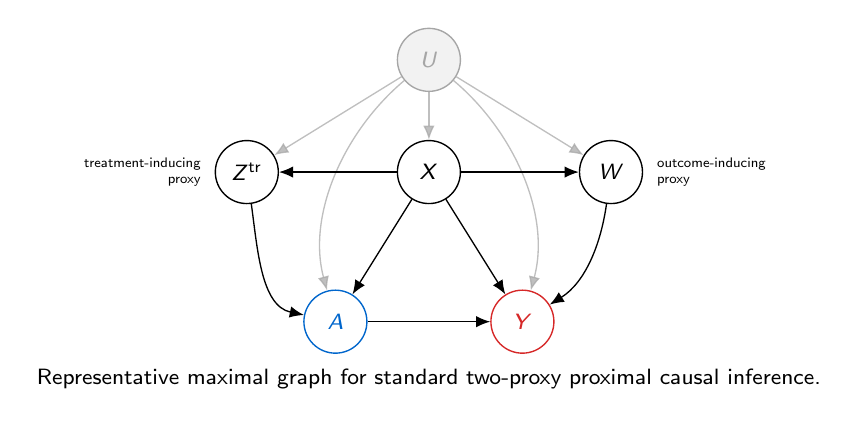
\begin{tikzpicture}[
  x=1.25cm,
  y=0.95cm,
  >={Latex[width=1.45mm,length=1.8mm]},
  font=\sffamily\sansmath\scriptsize,
  varnode/.style={draw,circle,inner sep=0mm,minimum size=8mm,
    line width=0.5pt,font=\sffamily\sansmath\footnotesize},
  observed/.style={varnode,draw=black,text=black,fill=white},
  latent/.style={varnode,draw=collatent,text=collatent,fill=filllatent},
  treatment/.style={varnode,draw=coltreat,text=coltreat,fill=white},
  outcome/.style={varnode,draw=colout,text=colout,fill=white},
  observed edge/.style={->,draw=black,line width=0.48pt},
  latent edge/.style={->,draw=collatent,opacity=0.72,line width=0.48pt}
]

\node[latent] (U) at (0,3.05) {$U$};
\node[observed] (Z) at (-1.85,1.55) {$Z^{\mathrm{tr}}$};
\node[observed] (X) at (0,1.55) {$X$};
\node[observed] (W) at (1.85,1.55) {$W$};
\node[treatment] (A) at (-0.95,-0.45) {$A$};
\node[outcome] (Y) at (0.95,-0.45) {$Y$};

\node[align=right,anchor=east,font=\sffamily\sansmath\tiny]
  at (-2.22,1.55) {treatment-inducing\\proxy};
\node[align=left,anchor=west,font=\sffamily\sansmath\tiny]
  at (2.22,1.55) {outcome-inducing\\proxy};

% Hidden confounding and proxy generation.
\draw[latent edge] (U) -- (X);
\draw[latent edge] (U) -- (Z);
\draw[latent edge] (U) -- (W);
\draw[latent edge] (U) to[out=220,in=105,looseness=0.90] (A);
\draw[latent edge] (U) to[out=320,in=75,looseness=0.90] (Y);

% Observed covariate effects.
\draw[observed edge] (X) -- (Z);
\draw[observed edge] (X) -- (W);
\draw[observed edge] (X) -- (A);
\draw[observed edge] (X) -- (Y);

% Proxy roles and treatment effect.
\draw[observed edge] (Z) to[out=-82,in=168,looseness=0.92] (A);
\draw[observed edge] (W) to[out=-98,in=32,looseness=0.92] (Y);
\draw[observed edge] (A) -- (Y);

\node[align=center,font=\sffamily\sansmath\footnotesize]
  at (0,-1.22) {Representative maximal graph for standard two-proxy proximal causal inference.};

\end{tikzpicture}
\end{document}
